\documentclass[12pt,a4paper]{article}

%\pdfoutput=1

\usepackage[utf8]{inputenc}
\usepackage[T1]{fontenc}
\usepackage[english]{babel}
\usepackage{amsmath}
\usepackage{mathabx}
\usepackage{lmodern}
\usepackage{listings}
\usepackage{units}
\usepackage{siunitx}
\usepackage{icomma}
\usepackage{graphicx}
\usepackage{caption}
\usepackage{subcaption}
\usepackage{color}
\usepackage{pgf}
\DeclareMathOperator{\acosh}{arccosh}
\newcommand{\N}{\ensuremath{\mathbbm{N}}}
\newcommand{\Z}{\ensuremath{\mathbbm{Z}}}
\newcommand{\Q}{\ensuremath{\mathbbm{Q}}}
\newcommand{\R}{\ensuremath{\mathbbm{R}}}
\newcommand{\C}{\ensuremath{\mathbbm{C}}}
\newcommand{\rd}{\ensuremath{\mathrm{d}}}
\newcommand{\id}{\ensuremath{\,\rd}}
\usepackage{hyperref}
%\usepackage{a4wide} % puts the page numbering further down the page.
\usepackage{pdfpages}
\usepackage{epstopdf}
\DeclareGraphicsExtensions{.eps}
\def\changemargin#1#2{\list{}{\rightmargin#2\leftmargin#1}\item[]}
\let\endchangemargin=\endlist

\title{Handin 2}
\author{Marcus Malmquist, marmalm, 941022}
\date{\today}

\begin{document}
\maketitle

\section{Task 1}\label{sec:1}
The beam waist is located at $z=0$ because that is how I define it. The beam width at $z=z_1$ (which is located at $z=-0.81$) is $\SI{296}{\micro\metre}$. Since the mirrors are separated by $\SI{95}{\centi\metre}$ and the left mirror is located at $z=-0.81$, the right mirror is naturally located at $z=0.14$.

\section{Task 2}\label{sec:2}
The beam width was numerically calculated to be $\SI{300}{\micro\metre}$ which is very close to the theoretical value. The theoretical value is more likely to be correct as it is theoretical (and if not it would just be rubbish). The simulation uses approximations (particularly when calculating the integral) which probaby has an inpact on the result.

\section{Task 3}\label{sec:3}
It is possible for a more incorrect and random starting field to converge into a the fundamental mode as seen in Figure~\ref{fig:task3}
\begin{figure}
  \centering
  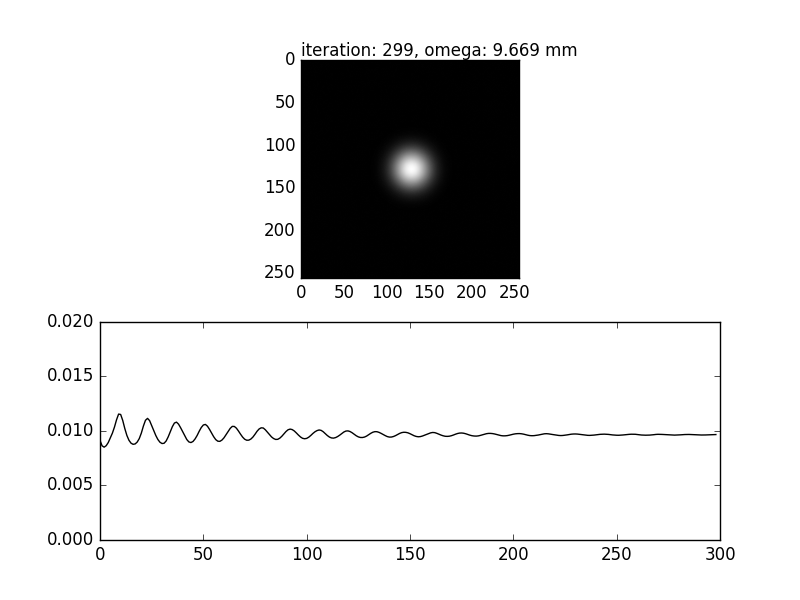
\includegraphics[width=\textwidth]{3_gauss_0_0.png}
  \caption{The gaussian beam after 300 iterations (top image) and the $e^{-2}$ radius (bottom graph)}
  \label{fig:task3}
\end{figure}

\section{Task 4}\label{sec:4}
The hair appears to turn the fundamental mode into a (0,1)-mode as can be seen in Figure~\ref{fig:task4} although it does not quite converge after 300 iterations.
\begin{figure}
  \centering
  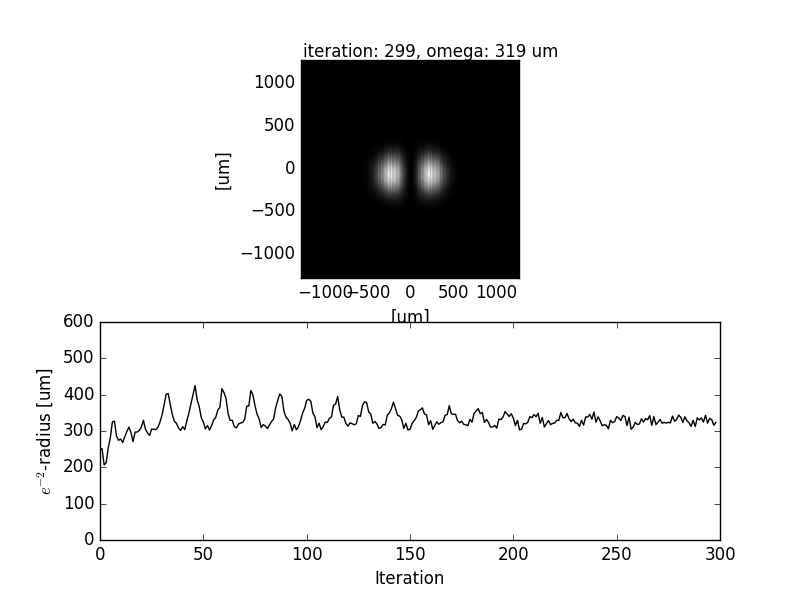
\includegraphics[width=\textwidth]{4_gauss_1_0.png}
  \caption{The gaussian beam after 300 iterations (top image) and the $e^{-2}$ radius (bottom graph). The bottom graph should only be used to judge wether or not the beam has converged.}
  \label{fig:task4}
\end{figure}

\section{Task 5}\label{sec:5}
Then hair appears to turn the fundamental mode into a (0,1)-mode as can be seen in Figure~\ref{fig:task5}. Item should be noted that it actually converges and it does so very quickly compared to the setup in Section~\ref{sec:4}.
\begin{figure}
  \centering
  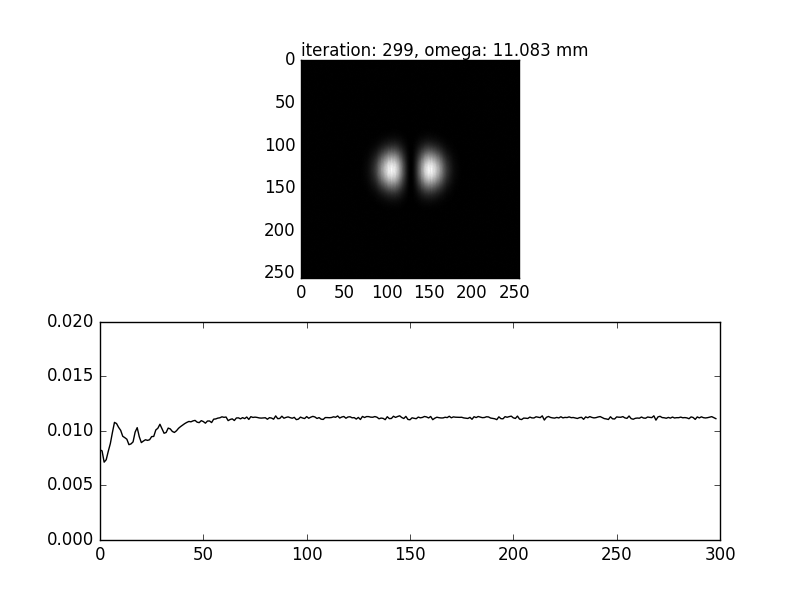
\includegraphics[width=\textwidth]{5_gauss_1_0.png}
  \caption{The gaussian beam after 300 iterations (top image) and the $e^{-2}$ radius (bottom graph). The bottom graph should only be used to judge wether or not the beam has converged.}
  \label{fig:task5}
\end{figure}

\section{Task 6}\label{sec:6}
The hairs appears to turn the fundamental mode into a (1,1)-mode as can be seen in Figure~\ref{fig:task6} although it does not quite converge after 300 iterations.
\begin{figure}
  \centering
  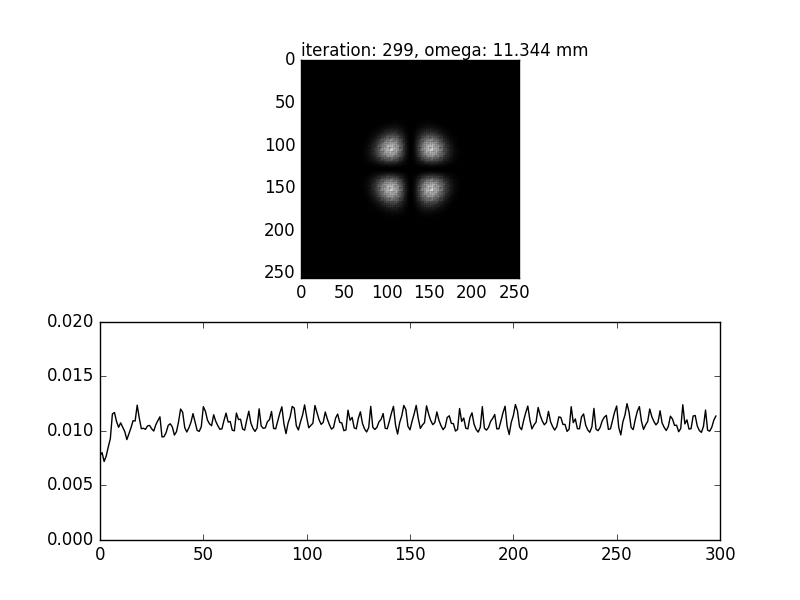
\includegraphics[width=\textwidth]{6_gauss_1_1.png}
  \caption{The gaussian beam after 300 iterations (top image) and the $e^{-2}$ radius (bottom graph). The bottom graph should only be used to judge wether or not the beam has converged.}
  \label{fig:task6}
\end{figure}

\section{Task 7}\label{sec:7}
\subsection{a}
Since we plot the intensity we loose information about the phase, which can cause the field (which has a phase) to look different when compared to the previous roundtrip.

\subsection{b}
Then graph in Figure~\ref{fig:task7b} confirms that the distance traveled in one roundtrip is not a multiple off $\lambda$. From the figure it seems that once the beam has converged the phase changes by just over $4\pi$ after three roundtrips.
\begin{figure}
  \centering
  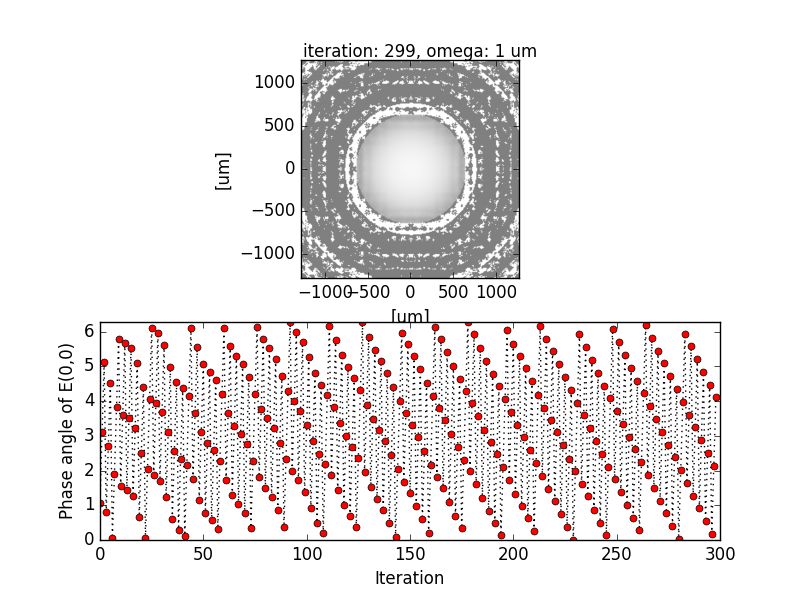
\includegraphics[width=\textwidth]{7b_gauss_0_0.png}
  \caption{The normalized phase of the gaussian beam after 300 iterations (top image) and the phase of $E(0,0)$ at the left mirror (bottom graph).}
  \label{fig:task7b}
\end{figure}

\subsection{c}
In order to make the phase of the field equal for two consecutive roundtrips one canadian change the distance between the mirrors slightly in order to make the distance traveled in one roundtrip be a multiple offset $\lambda$.
\newpage
\appendix
\section{Code}
\begin{changemargin}{-3cm}{0.5cm}
\lstinputlisting[language=Python]{tsm.py}
\end{changemargin}
\end{document}